\chapter{A full life cycle Dynamic Energy Budget (DEB) model for Peruvian anchovy \textit{Engraulis ringens} in the northern Humboldt Current system (NHCS)}\label{Chap4}

\clearpage
\section*{Abstract}
A comprehensive Dynamic Energy Budget (DEB) model for the Peruvian anchovy (\textit{Engraulis ringens}) has been developed. The model parameters were estimated from larval length growth data at different temperatures obtained from laboratory experiments, as well as from Von Bertalanffy growth curves for juveniles and adults. The model was able to reproduce well the observed patterns of larval, juvenile, and adult growth, as well as the physiological characteristics of the species, including the age at hatching (first feeding), age at metamorphosis (end of growth acceleration), and age at puberty (onset of reproductive activity). The length-weight relationship and the relationship between length and number of oocytes were also well represented. A simulation experiment demonstrated that \textit{E. ringens} exhibits a physiological advantage over \textit{E. encrasicolus} when subjected to a feeding deprivation process for small larvae ($0.5 cm$), whereas this characteristic is reversed for larger larvae ($3 cm$). The age at birth for both species would be similar, but a difference is evident when considering the age at metamorphosis. In this context, \textit{E. ringens} would exhibit accelerated growth for a longer period than \textit{E. encrasicolus}. However, there would be a critical temperature threshold above 21 \textdegree C, after which, the individuals would not succeed in reaching later stages of their development. Finally, \textit{E. ringens} would initiate reproductive activity later than its European counterpart.\\

Keywords: DEB model, growth acceleration, \textit{E. ringens}

\clearpage
\section{Introduction}

The \acrfull{deb} theory has been successfully applied to several marine species that are important for fisheries worldwide by taking individuals as dynamic systems, considered as the basic level of metabolic organization, relatively easy to make energy and mass balances allowing us to model the allocation of energy and nutrients in living organisms through its entire life cycle \citep{Kooi2009}.\\

Marine fish have complex life cycles that consist of distinct developmental stages, including eggs, larvae, juveniles, and adults \citep{Pepi1991,LikaKooi2014}. The duration of each stage varies depending on the species and the environment surrounding each individual. This variation has been documented in studies by \cite{GreeFish2004}, and \cite{FontSant2011}.\\

When describing the life cycle of a fish using a mechanistic model, it is generally assumed that isomorphic growth occurs. This growth is often modeled using a von-Bertalanffy growth model, which can reproduce general growth patterns focusing on juvenile and adult stages, as growth data for these stages are more accessible for modeling \citep{VonB1957,MarzShin2009}. However, during early life stages, non-isomorphic development has been observed in different anchovy species \citep{PaloMora1988,TakaWata2001,MoreClar2011} and other reported teleost fish species \citep{KlinFros1991,OsseVan1995,LikaKooi2014}. Thus, to accurately describe the growth patterns of the early life stages (eggs and larvae), it is necessary to consider the acceleration of growth during these stages, well modeled by a Gompertz curve \citep{Gomp1825,KooiPecq2011}. This modelling approach, an extension of the standard \acrshort{deb} model ($DEB_{std}$), which we will refer to from now on as $DEB_{abj}$, has already been used when studying similar species to the Peruvian anchovy \citep{PecqPeti2009,GattPeti2017,MenuPecq2023}. Also, when \acrshort{deb} theory has been coupled with \acrshort{ibm}, has proven useful in shedding light on phenomena that are difficult to test in natural environments, such as larval growth influenced by the environment \citep{MartZimm2012,DaviJoac2019,BuenPeti2020,FlorLett2023} or complex fish population patterns arising from individual behavioral responses to their environment \citep{MartJage2013,BeauGous2015,BrocAuge2018,LiuZhan2023}.\\

Then, the aims of this chapter/article/paper is to produce the first \acrshort{deb} model for Peruvian anchovy (\textit{\gls{ringens}}), with a specific set of parameters estimated  that includes growth acceleration ($DEB_{abj}$) during the larval period to metamorphosis. Chapter \ref{Chap5} will present a practical use of the growth parameters of \textit{\gls{ringens}} in the study of early life stages off Peru.\\

\clearpage
\section{Methods}\label{Chap4Meth}

\subsection{DEB-model formulation}\label{Chap4MethDEBformulation}

A \acrshort{deb} accelerated growth model ($DEB_{abj}$) is derived from a standard growth model ($DEB_{std}$). A $DEB_{std}$ model explains how an organism uses energy for maintenance, growth, and reproduction based on its state and environment, such as food density and temperature. The $DEB_{std}$ model deals with one type of food, reserve, and structure for an isomorph, which is an individual that maintains the same shape (surface-to-volume ratio) during growth \citep{Kooi2009}, nevertheless, it should be noted that not all living beings exhibit this characteristic throughout their life cycle.\\

$DEB_{std}$ describes an individual based on three state variables: reserve energy ($E$), structural volume ($V$) and reproduction buffer ($E_{R}$). An organism obtains energy from food by assimilation ($\dot{p}_{A}$), the process that transforms food into reserves ($E$), defined as a collection of metabolizable compounds that have the potential to fuel all metabolic processes of an individual and it is directly influenced by changes in food availability in the environment and does not require energy expenditure for maintenance. Reserve is continuously used and replenished, while structural material is continuously degraded and reconstructed as a result of somatic maintenance. Assimilation is taken to be proportional to the surface-area of the structural volume and maintenance is taken to be proportional to structural volume. Ingestion is assumed to follow a functional response relationship with food density and to be proportional to the structural surface area. The scaled (dimensionless and Holling type-II) functional response ($f$) ranges from 0 (starvation) to 1 (``ad libitum''). After assimilation, energy is mobilized ($\dot{p}_{C}$) and used for growth ($\dot{p}_{G}$), specifically the increase of structure ($V$), a fixed fraction of the mobilized reserve after subtracting for somatic maintenance ($\dot{p}_{S}$) which takes priority over growth and is proportional to structure. Parameters related to metabolic rates are temperature-dependent but remain constant otherwise, relative to a reference temperature $T_{1}$.\\

One of the fundamental principles of \acrshort{deb} theory is homeostasis, a mechanism that serves to maintain the internal conditions of an organism in a state of equilibrium, even in the face of environmental fluctuations. This is exemplified by the relatively constant chemical composition of the body, which is observed in fish as well \citep{Kooi2009}. Consequently, the chemical composition of the reserve and structure remains constant, although their ratio may fluctuate, thereby influencing the chemical composition of the entire body. If the environmental conditions remain relatively stable, the composition of the entire fish remains constant. The \acrshort{deb} model assumes that the reserve will be continuously used and refilled, while somatic maintenance will continuously reduce and rebuild structural material throughout the individual's life. Energy is allocated to structure and maturation/reproduction only after maintenance costs have been paid, which means, \acrshort{deb} models prioritize the metabolic cost of individual survival through somatic maintenance over growth and reproduction \citep{Kooi2009,JusuSous2017}.\\

\subsubsection{Non-isomorphic growth acceleration hypothesis}

A change in the shape (surface-to-volume ratio) during a specific life stage is referred to as ``growth acceleration''. This metabolic acceleration is confined between the energy thresholds (which may or may not correspond to changes in morphology) at birth ($E_H^b$) and (metabolic) metamorphosis ($E_H^j$), during which maximum specific assimilation ($\left [ \dot{p}_{M} \right ]$) and energy conductance ($\dot{v}$) increase with length \citep{KooiLika2014}, based on the growth acceleration hypothesis \citep{OsseBoog1997,JohnBjor2001,WalkMcCo2004,PaulFroe2023}. In this particular case, we are talking about an accelerated \acrshort{deb} model ($DEB_{abj}$, Fig. \ref{Chap4DEBfluxbox}) which is an extension of the standard model and includes the concept of maturity ($E_{H}$), that refers to the level of development of an organism. This fourth new state variable, provides information on the maturity state of the individual, as energy or mass invested in maturation is dissipated in the form of heat or metabolites \citep{JusuKlan2011}.

\begin{figure}[ht]
	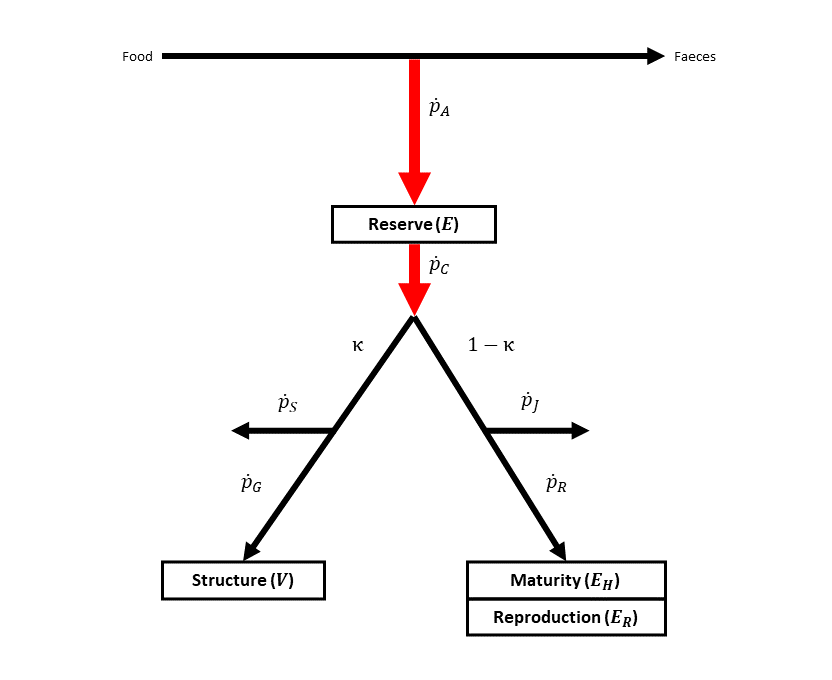
\includegraphics[width=1.0\textwidth]{figures/Chap4DEBfluxbox.png}
	\centering
	\caption{Main metabolic processes of DEB theory. The diagram depicts state variables as boxes and energy fluxes as arrows respectively. Red thicker arrows indicate the process of growth acceleration in the assimilation ($\dot{p}_{A}$) and mobilization ($\dot{p}_{C}$) flows until metamorphosis is reached. Other flows, somatic maintenance ($\dot{p}_{S}$), maturity maintenance ($\dot{p}_{J}$), growth ($\dot{p}_{G}$), maturation/reproduction ($\dot{p}_{R}$), are not affected by acceleration. Constant fraction of ($\dot{p}_{C}$) allocated to somatic maintenance and growth ($\kappa$) and the remaining fraction ($1-\kappa$) for maturity and reproduction.}
	\label{Chap4DEBfluxbox}
\end{figure}

For early developmental stages, the concept of maturity helps us to define the process of accelerated growth during the larval period until metabolic metamorphosis, period in which the shape coefficient ($\delta_{M} = \delta_{larvae}$) will be dynamic and defined by equation \ref{shape_dinam}, where $E_{H(i)}$ will be a value that changes at each time step ($i$). After metabolic metamorphosis, the shape coefficient ($\delta_{M} = \delta_{adult}$) will again be a fixed value.\\

\begin{equation}
	\delta_M = \frac{\delta_{larvae} (E_H^j - E_{H(i)}) + \delta_{adult} (E_{H(i)} - E_H^b)}
	{E_H^j - E_H^b}
	\label{shape_dinam}
\end{equation}\\

It is useful to understand the difference between morphological life stages and functional life stages. Morphological life stages are assigned based on a description of the species or group, in our case, fish. A single model captures the entire life cycle from conception to death, and transitions (embryo, juvenile, adult) between functional life stages are constructed as (metabolic) switches. The embryo grows, matures, but does not feed; juveniles grow, mature, feed, but are not ready to reproduce, an exclusive characteristic of adults. Type $DEB_{abj}$ has never been found in cartilaginous fish, amphibians, reptiles, birds or mammals, and typically occurs in taxa with larval stages.\\

In addition, the embryonic stage ends with an energetic maturity threshold at birth ($E_{H}^{b}$, first feeding) using only reserves to grow and develop ($\dot{p}_{A} = 0$). After assimilation, energy is mobilized ($\dot{p}_{C}$) and used for growth ($\dot{p}_{G}$), specifically the increase of structure ($V$), a fixed fraction of the mobilized reserve after subtracting for somatic maintenance ($\dot{p}_{S}$) which takes priority over growth and is proportional to structure. The increase in this structure depends on the levels of reserve and structure and requires a continuous maintenance cost. In this context, the maturity level ($E_{H}$) increases when the remaining fraction of mobilized reserve is allocated to processes other than maturity maintenance ($\dot{p}_{J}$).\\

Between birth and metamorphosis, the individual's metabolic processes will be affected by temperature ($C_{T}$) and an acceleration factor ($S_{M}$). Additionally, two new parameters related to energy conductivity ($V$) and the maturity maintenance rate coefficient ($k_{j}$) were included. Stage transitions are modeled by increasing the level of maturity from zero to a maximum value and defining threshold levels at which transitions take place. At $E_{H} = E_{H}^{b}$, an embryo transitions to a larva, at $E_{H} = E_{H}^{j}$, it metamorphoses into a juvenile, and at $E_{H} = E_{H}^{p}$.\\

Upon reaching adulthood, the level of maturity ceases to increase as the energy is redirected towards reproduction ($\dot{p}_{R}$), allocating energy to $E_{R}$, which has a value equal to zero until before reaching the adult stage. A constant fraction ($\kappa$) of the mobilized energy from reserve is allocated to maturity maintenance and reproduction. In adults, if there is no food assimilation because of starvation the reproductive buffer is utilized to pay maintenance costs \citep{BrosLlor2016,GattPeti2017,MenuPecq2023}.\\

\subsection{\textbf{$DEB_{abj}$} equations and how they differ from \textbf{$DEB_{std}$}}

Since $DEB_{abj}$ is an extension of the standard version ($DEB_{std}$), most of the equations are the same as described in Chapter \ref{Chap3}. These differences will then be implemented to couple the $Ichthyop-DEB_{abj}$ model.

Jorge Flores-Valiente et al.\\

\subsubsection{Forcing variables}\label{Chap4ForVar}
\hfill \\

$T$ Temperature ($K$) is the water temperature surrounding an individual in which \textit{\gls{ringens}} larvae were reared \citep{RiouOfel2021} and the temperature associated with the von Bertalanffy growth parameters \citep{PaloMuck1987}. Feeding conditions were \textit{ad libitum}, so we assumed a constant value for the functional response ($f = 1$).\\

\subsubsection{Initial conditions of state variables (egg stage)}\label{Chap4InitCond}

The age of the individual is set at zero on the day of spawning.\\

\begin{tabular}{|c|c|c|c|}
\hline 
Symbol  & Value      & Units  & Definition      \\ 
\hline 
$E$     & $0.99$     & $J$    & Initial Reserve \\ 
$V$     & $0.000001$ & $mm^3$ & Initial Structure\\
$E_{H}$ & $0$ 		  & $J$    & Cumulated energy invested into development\\
$E_{R}$ & $0$         & $J$   & Reproduction buffer\\
\hline 
\end{tabular}

\subsubsection{Primary parameters}\label{Chap4PriPar}
Table \ref{param_compar} below shows the comparison of parameters used by the $DEB_{std}$ and $DEB_{abj}$ models for \textit{\gls{encrasicolus}} and \textit{\gls{ringens}}, respectively.

\subsubsection{Scaled functional response}\label{Chap4resp_f}
Same as section \ref{Chap3resp_f}

\subsubsection{Temperature correction}\label{Chap4cT_corr}
Same as section \ref{Chap3cT_corr}, but then, temperature correction affects two additional parameters.\\

$\dot{v}_{T} = C_{T} \dot{v}_{T_{1}}$\\

$\dot{K}_{jT} = C_{T} \dot{K}_{jT_{1}}$\\

\subsubsection{Metabolic acceleration}\label{Chap4Acc}
\hfill \\

Only two parameters are impacted by growth acceleration.\\

\textbf{if}	$E_{H} < E_{H}^b$\\

$S_{M} = 1$ \hfill No acceleration.\\

\textbf{else if} $E_{H}^b < E_{H} < E_{H}^j$\\

$S_{M} = \frac{L}{L_{b}}$ \hfill Acceleration.\\

\textbf{else}\\

$S_{M} = \frac{L_{j}}{L_{b}}$ \hfill Constant growth.\\

The $S_{M}$ parameter only accelerates growth from birth to metamorphosis.\\

$\left \{ \dot{p}_\mathrm{Am} \right \}_{S_{M}} = S_{M} \left \{ \dot{p}_\mathrm{Am} \right \}_{T}$\\

$\dot{v}_{S_{M}} = S_{M} \dot{K}_{jT}$\\

\subsubsection{Fluxes ($Jd^{-1}$)}\label{Chap4Fluxex}
\hfill \\

\textbf{if}	$E_{H} < E_{H}^b$\\

$\dot{p}_\mathrm{A} = 0$ \hfill No assimilation.\\

\textbf{else}\\

$\dot{p}_\mathrm{A} = f \left \{ \dot{p}_\mathrm{Am} \right \}_{S_{M}} V^{2/3}$ \hfill Assimilation.\\

\hfill \\

$\dot{p}_\mathrm{M} = \left [ \dot{p}_{M} \right ]_{T} V$ \hfill Volume-related somatic maintenance.\\

$\dot{p}_{C} = \frac{E}{V}*\frac{\left [ E_{G} \right ]\dot{v}_{S_{M}}V^{2/3}+\left [ \dot{p}_{M} \right ]_{T}}{\kappa\frac{E}{V}+\left [ E_{G} \right ]}$ \hfill Mobilization of energy.\\

$\dot{p}_{J} = \dot{K}_{jT} E_{H}$ \hfill Maturity maintenance.\\

\subsubsection{Differential equations}\label{Chap4DiffEq}
Same as section \ref{Chap3DiffEq}, and additionally.

\textbf{if} $E_{H} < E_{H}^p$\\

$\frac{dE_{H}}{dt} = (1 - \kappa) \dot{p}_{C} - \dot{p}_{J}$\\

$\frac{dE_{R}}{dt} = 0$\\

\textbf{else}\\

$\frac{dE_{H}}{dt} = 0$\\

$\frac{dE_{R}}{dt} = (1 - \kappa) \dot{p}_{C} - \dot{p}_{J}$\\

\subsubsection{Integration}\label{Chap4Integ}
Same as section \ref{Chap3Integ}, and additionally.

$E_{H}\left ( t + \Delta t \right ) = E_{H}\left ( t \right ) + \frac{dE_{H}}{dt}\Delta t$ \\

$E_{R}\left ( t + \Delta t \right ) = E_{R}\left ( t \right ) + \frac{dE_{R}}{dt}\Delta t$ \\

With $\Delta t = 0.083 d \left (=2hours\right )$

\subsubsection{Observable variables}\label{Chap4ObsVar}
Same as section \ref{Chap3ObsVar}, and additionally, $\delta_{M}$ is calculated as in eq. \ref{shape_dinam}.

\subsection{Data sources and parameter estimation}

The simultaneous integration of disparate data sources, each exhibiting varying degrees of quality, often proves to be a significant challenge when attempting to obtain or estimate model parameters. It is here that our data collection is based on a specific data source model, a ``zero-variate'' data concerning a single value associated to a variable and ``uni-variate'' data, associated to a set of paired numbers \citep{MarqLika2019}. Fig. \ref{Chap4AmP_flow} details the flow chart of the Add my Pet ($AmP$) project parameter estimation and the full details process can be found in \cite{MarqAugu2018}. This method minimizes the sum of squared deviations between model predictions and observations, with weight coefficients set to equal the inverse squared data to remove unit effects.\\

\begin{figure}[ht]
	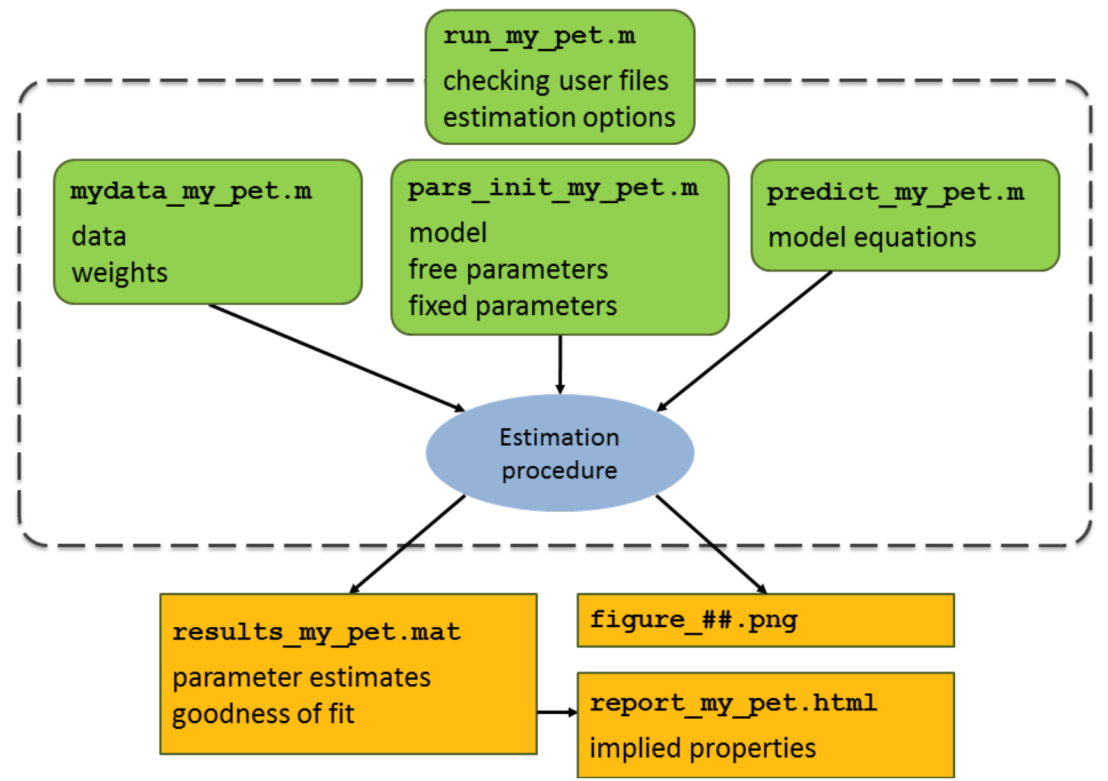
\includegraphics[width=1.0\textwidth]{figures/Chap4AmP_flow.png}
	\centering
	\caption{The architectural framework of the $AmP$ tool is presented. Green rectangles represent user-defined files, specifically: \textbf{$run\_my\_pet$} (run a parameter estimation), \textbf{$mydata\_my\_pet$} (for zero-variate and uni-variate data collection), \textbf{$pars\_init\_my\_pet$} (for the initial values of the parameters to be estimated), and \textbf{$predict\_my\_pet$} (to specify details of parameter estimation). The orange rectangles represent the output. ``\textbf{$my\_pet$}'' refers to the species in question that is the reason for parameter estimation. Figure taken from \citep{MarqAugu2018}.}
	\label{Chap4AmP_flow}
\end{figure}

\subsubsection{Zero-variate data}

Table \ref{zero-variate} presents the data collection for \textbf{\gls{ringens}} which includes information on age ($d$), standard length ($cm$), total length ($cm$), weight ($g$), and reproductive activity ($\#/d$). In addition, variables concerning initial conditions such as the volume of an egg ($cm^3$) and its energy content ($J$) are presented.\\

The age at hatching ($a_{h}$) was estimated at 2,288 $days$, while the time elapsed from hatching to birth ($t_{b}$, understood as the age at the first feeding of the individual) was calculated at 3,805 $days$. Metabolic metamorphosis ($t_{j}$, cessation of growth acceleration) occurs 65.34 $days$ after hatching. The age at puberty ($t_{p}$), when the individual begins to accumulate energy for reproductive purposes, would be reached at 274.8 $days$ after birth (first feeding). Given that this species does not typically live for a long period of time, it was postulated that its lifespan ($a_{m}$	) would be equivalent to 1,540 $days$. The initial energy content ($E0$) of an engraulid egg is assumed to be close to 1 $J$ ($\sim$0.9672 $J$) while its initial volume ($V0$, structure) is estimated to be close to zero (0.0002285 $cm^3$).\\

In the case of lengths ($cm$), it can be observed that the available data employs two distinct measures: the standard length and the total length. To address this issue, a relationship between the two measurement types has been proposed, based on a correlation observed in \href{https://www.fishbase.se/summary/Engraulis-ringens.html}{Fishbase}, as shown in equation \ref{LS_LT}, where $TL = Total\: length$ and $SL = Standard\: length$.

\begin{equation}
	TL = 1.141 (SL) 
	\label{LS_LT}
\end{equation}\\

The standard length at hatching ($L_{h}$) was estimated to be 0.2971 $cm$, while the standard length at yolk absorption ($L_{b}$) was estimated at 0.5499 $cm$. Subsequently, the organism undergoes a rapid growth phase, reaching a length of 1.583 $cm$ at the point of metabolic metamorphosis ($L_{j}$). When the individual reaches 11.13 $cm$, it begins to accumulate energy for reproduction ($L_{p}$) and continues to grow up to 20 $cm$, when it reaches its ultimate length ($L_{i}$) and its ultimate wet weight ($W_{wi}$,85 $g$). Once the individual begins to accumulate energy for reproduction, it reaches a maximum daily reproduction rate ($Ri$) of 2145 oocytes ($\#/d$) with a strategy of 20 spawnings per year (communication with experts).\\

The last seven parameters in the Table \ref{zero-variate} refer to pseudo data ($psd.$), which help in parameter estimation, giving a weight to a specific variable when performing a Ballesian statistical estimation.\\

\subsubsection{Uni-variate data}

The uni-variate data (Table \ref{uni-variate}) refer to laboratory larval rearing experiments at two temperatures (Fig. \ref{Chap4LarvaDataVSModel}, blue line: 14.5 \textdegree C and red line: 18.5 \textdegree C), both under conditions of total food satiation ($f=1$), where age is expressed in days after hatching ($d$) and standard length in centimeters ($cm$) \citep{RiouOfel2021}. Using von Bertalanffy growth parameters \citep{PaloMuck1987}, (Fig. \ref{Chap4AdultDataVSModel}) point data were obtained for the average 4-year life span of \textit{\gls{ringens}} where age is expressed in days since birth ($d$,first feeding) and total length in centimeters ($cm$).\\

The length-weight ratio (Fig. \ref{Chap4LengthVSWeight}) includes individuals from 12 to 17 $cm$ with a weight range between 10 and 45 grams ($g$). These data were obtained from the literature \citep{Mina1968} while the data on fecundity (Fig. \ref{Chap4LengthVSOocytes}) come from surveys conducted by IMARPE, and correspond to the relationship between the length ($cm$) and the number of oocytes per batch ($\#$) \citep{PereBuit2000}.

\clearpage
\section{Results}

\subsection{Zero-variate and univariate data prediction}

The fully parameterized $DEB_{abj}$ model exhibits a high degree of accuracy to the characteristics observed in the existing dataset on \textit{\gls{ringens}}. A comparison of the zero-variate data in Table \ref{zero-variate} indicates a satisfactory correspondence between the model predictions and observations. The embryonic stage of development is particularly well captured by aspects of early development, including the age at hatching ($a_{h}$), egg volume ($V0$), caloric value of the egg ($E0$), and standard length at hatch ($L_{h}$), with a low relative error value. Age at birth after hatch ($t_{b}$) and length at birth ($L_{b}$, standard length at yolk-absorption, understood as the time at which the individual initiates food intake) were also well represented by the model. Given that the age and standard length of metamorphosis ($t_{j}$, $L_{j}$) data for \textit{\gls{ringens}} are related to changes in morphology and not to an energy threshold, the model predictions exhibit a slight variation from the data. The age at which puberty begins ($t_{p}$), understood as the time at which the individual begins to accumulate energy for reproduction, varies relatively with respect to the data. However, total length at puberty ($L_{p}$) is closer to the data source. The model also demonstrated an accurate representation of the life spam ($a_{m}$) and ultimate total length ($L_{i}$) as well as the ultimate wet weight ($W_{wi}$). The maximum reproduction rate ($R_{i}$) slightly overestimated the values with respect to the data source.\\

The patterns of larval growth, adult growth, length-weight and length-oocyte relationships (uni-variate data source, Table \ref{uni-variate}) were accurately reproduced by the \acrshort{deb} parameter set estimated for \textit{\gls{ringens}} (Table \ref{param_compar}). The model successfully captures the acceleration of growth rate in the larval stage, especially up to 30 $days$ after hatching (Fig. \ref{Chap4LarvaDataVSModel}), which increases by a factor of 4.5 when individuals are exposed to a temperature of 18.5 \textdegree C (from 0.3 $cm$ to nearly 1.5 $cm$) and by a factor of 1.8 when individuals are exposed to a temperature of 14.5 \textdegree C (from 0.6 $cm$ to nearly 1.1 $cm$). Adult growth was also well represented reaching asymptotic growth at about 18.5 $cm$ (Fig. \ref{Chap4AdultDataVSModel}).\\

In the adult phase, the length-weight relationship showed an allometric relationship of xx (\textbf{ask for the blue curve equation}) (Fig. \ref{Chap4LengthVSWeight}) while we observed in Fig. \ref{Chap4LengthVSOocytes} that the number of oocytes ($\#$) increased in direct proportion to the total length ($cm$).\\

%\begin{landscape}
\begin{table}[H]
\centering
\begin{adjustbox}{width=1.0\textwidth}
\small
\begin{NiceTabular}{r|r|r|c|c|l|r|r}
\hline
\multicolumn{1}{c}{\textbf{Data}}				&
  \multicolumn{1}{c}{\textbf{Prediction}}		&
  \multicolumn{1}{c}{\textbf{Relative error}}	&
  \multicolumn{1}{c}{\textbf{Symbol}}			&
  \multicolumn{1}{c}{\textbf{Units}}			&
  \multicolumn{1}{c}{\textbf{Description}}		&
  \multicolumn{1}{c}{\textbf{Reference}}		&
  \multicolumn{1}{c}{\textbf{Weights}}			\\
\hline
\multicolumn{8}{c}{\textbf{Zero-variate data}}	\\
\hline
2.3						&
2.288					&
0.005302				&
$a_{h}$					&
$d$						&
Age at hatching			&
\cite{WareMend1981}		&
-						\\
4.4								&
3.805							& 
0.1353							& 
$t_{b}$							& 
$d$								& 
Time at birth since hatching	&
\cite{WareMend1981}				&
-								\\
80                                       & 
65.34                                    &
0.1833                                   & 
$t_{j}$                                  &
$d$                         			  &
Time since hatching at end metamorphosis &
\cite{MoreClar2011} 					  &
-										  \\
365           				 	& 
274.8          				 	& 
0.2472   					 	& 
$t_{p}$           			 	& 
$d$                        	 	& 
Time since birth at puberty		&
\cite{MarzShin2009}			 	&
-								\\
1460				 	& 
1540				 	& 
0.05478				 	& 
$a_{m}$				 	& 
$d$						& 
Life span				&
\cite{MarzShin2009}		&
-						\\
1					&
0.9672				&
0.03285				&
$E0$				&
$J$					&
Egg energy content	&
-					&
-					\\
0.00033					& 
0.0002285				& 
0.3077					& 
$V0$					& 
$cm^3$					&
Egg volume				&
\cite{RiouOfel2021}		&
-						\\
0.3							& 
0.2971						& 
0.009804					& 
$L_{h}$						& 
$cm$						& 
Standard length at hatch	&
\cite{RiouOfel2021}			&
-							\\
0.4													&
0.5499												& 
0.3746												& 
$L_{b}$												& 
$cm$												& 
Standard (notocordal) length at yolk-absorption	&
\cite{WareMend1981}									&
-													\\
3									& 
1.583								& 
0.4724								& 
$L_{j}$								& 
$cm$								& 
Standard length at metamorphosis	&
\cite{MoreClar2011}					&
-									\\
10							&
11.13						& 
0.113						& 
$L_{p}$						& 
$cm$						&
Total length at puberty		&
\textit{search bib}			&
-							\\
19                    &
23.55                 & 
0.2393                & 
$L_{i}$               & 
$cm$                  &
Ultimate total length &
\cite{MarzShin2009}   &
-					   \\
56                  &
85.7                &
0.5304              &
$W_{wi}$            & 
$g$                 & 
Ultimate wet weight &
\cite{PaloMuck1987} &
-					 \\
1644						& 
2145						& 
0.3047						& 
$Ri$						& 
$\#/d$						& 
Maximum reproduction rate	&
\cite{PereBuit2000}			&
-							\\
0.02					& 
0.04124					& 
1.062					& 
$psd.v$					& 
$cm/d$					& 
Energy conductance		&
-						&
-						\\
18                           		& 
80.71                        		& 
3.484                        		& 
$psd.p_{M}$                  		& 
$J/dcm^3$ 					  		& 
Vol-specific somatic maintenance	&
-							  		&
-							  		\\
0.002                           		&
0.002                           		&
0                               		&
$psd.k_{J}$                        		&
$1/d$                      		 		&
Maturity maintenance rate coefficient  &
-										&
-										\\
0.3					&
0.1112				&
0.6294				&
$psd.k$				&
$1/d$				&
Maintenance ratio	&
-					&
-					\\
0.8								& 
0.5512							& 
0.311							& 
$psd.kap$						&
-								& 
Allocation fraction to soma		&
-								&
-								\\
0.8					& 
0.7919				& 
0.01008				& 
$psd.kap_{G}$		& 
-					& 
Growth efficiency	&
-					&
-					\\
0.95                   		&
0.95                   		&
0                      		&
$psd.kap_{R}$          		& 
-                      		&
Reproduction efficiency		&
-							&
-							\\
\hline
\end{NiceTabular}
\end{adjustbox}
\caption{List of zero-variate data and their estimated values. The relative error, symbol, physical units used in the model, and the description of each parameter are shown. The parameters obtained from the bibliography are accompanied by their respective references. The label ``$psd.$'' indicates a parameter used as a pseudo-data and gives particular ``weight'' when using Bayesian statistical estimation.} 
\label{zero-variate}
\end{table}
%\end{landscape}

%\begin{landscape}
\begin{table}[ht]
\centering
\begin{adjustbox}{width=1.0\textwidth}
\small
\begin{NiceTabular}{r|r|r|c|c|l|r|r}
\hline
\multicolumn{1}{c}{\textbf{Data}}				&
  \multicolumn{1}{c}{\textbf{Prediction}}		&
  \multicolumn{1}{c}{\textbf{Relative error}}	&
  \multicolumn{1}{c}{\textbf{Symbol}}			&
  \multicolumn{1}{c}{\textbf{Units}}			&
  \multicolumn{1}{c}{\textbf{Description}}		&
  \multicolumn{1}{c}{\textbf{Reference}}		&
  \multicolumn{1}{c}{\textbf{Weights}}			\\
\hline
\multicolumn{8}{c}{\textbf{Uni-variate data}}	\\
\hline
see										 &
Fig. \ref{Chap4LarvaDataVSModel}		 &
0.136									 & 
$tL_{larvHighT}$						 &
-										 &
Time since hatching vs. Standard length &
\cite{RiouOfel2021}						 &
-		                                \\
see										 &
Fig. \ref{Chap4LarvaDataVSModel}		 &
0.1237									 & 
$tL_{larvLowT}$							 &
-										 &
Time since hatching vs. standard length &
\cite{RiouOfel2021}						 &
-										 \\
see									&
Fig. \ref{Chap4AdultDataVSModel}	&
0.03565								&
$tL$								&
-									&
Time since birth vs. Total length  &
\cite{PaloMuck1987}					&
-									\\
see										 &
Fig. \ref{Chap4LengthVSWeight}			 &
0.07149									 & 
$LW$							 		 &
-										 &
Total length vs. Total weight			 &
\cite{Mina1968}							 &
-		                                \\
see											  &
Fig. \ref{Chap4LengthVSOocytes}			 	  &
0.2525									 	  & 
$LN_2$									 	  &
-										 	  &
Total length vs. Number of oocytes per batch &
\cite{PereBuit2000}						 	  &
-		                                	  \\
\hline
\end{NiceTabular}
\end{adjustbox}
\caption{Same as table \ref{zero-variate}, but for uni-variate data.} 
\label{uni-variate}
\end{table}
%\end{landscape}

%\begin{landscape}
\begin{table}[ht]
\centering
\begin{adjustbox}{width=1.2\textwidth}
\begin{tabular}{c|c|c|c|l|c|c}
\hline
Symbol																&
\makecell[c]{\textit{E. encrasicolus} \\ {\cite{PethRoos2013}}}	&
\textit{E. ringens}													&
Unit																&
Definition															&
Free																&
\makecell[c]{Reference \\ \textit{E. ringens}}															\\
\hline
$L_{1}$			&
0.28			&
-				&
$cm$			&
Hatch length	&
-				&
$AmP$			\\
$L_{2}$						&
0.35						&
-							& 
$cm$						& 
Length at first-feeding		& 
-							&
$AmP$						\\
$E_{H}^{b}$						& 
-								& 
0.335							& 
$J$								& 
Maturity threshold at birth		& 
-								&
$AmP$							\\
$E_{H}^{j}$								&
-										& 
83.22									& 
$J$										& 
Maturity threshold at metamorphosis		& 
-										&
$AmP$									\\
$E_{H}^{p}$						& 
-								& 
42160							& 
$J$								& 
Maturity threshold at puberty	& 
-								&
$AmP$							\\
$L_{b}$												& 
-													& 
0.1038												& 
$cm$												& 
Volumetric length at birth (estimated at $f$ = 1)	& 
-													&
$AmP$												\\
$L_{j}$														& 
-															& 
0.6093														& 
$cm$														& 
Volumetric length at metamorphosis (estimated at $f$ = 1)	& 
-															&
$AmP$														\\
$T_{A}$					& 
9800					& 
10000					& 
$K$						& 
Arrhenius temperature	& 
-						&
$AmP$					\\
$T_{L}$						&
279							&
279							&
$K$							&
Lower temperature boundary	&
-							&
$AmP$						\\
$T_{H}$						&
294(297)					& 
294(297)					& 
$K$							& 
Upper temperature boundary	& 
-							&
$AmP$						\\
$T_{AL}$									& 
20000										& 
20000										& 
$K$											& 
Arrhenius temperature for lower boundary	&
-											&
$AmP$										\\
$T_{AH}$									& 
95000(570000)								& 
95000(570000)								& 
$K$											& 
Arrhenius temperature for upper boundary	& 
-											&
$AmP$										\\
$\kappa_{\mathrm{x}} $						& 
0.71										& 
0.8											& 
-											& 
Fraction of food energy fixed in reserve	&
-											&
$AmP$										\\
$\left \{ \dot{p}_\mathrm{Xm} \right \}$								&
516																		& 
$\left \{ \dot{p}_\mathrm{Am} \right \}/\kappa \mathrm{x} = 106(622)$	& 
$J.cm^{-2}.d^{-1}$														& 
\makecell[l]{Maximum surface specific ingestion rate \\ (before and after metamorphosis for \textit{E. ringens})}																&
-																		&
$AmP$																	\\
$\left \{ \dot{p}_\mathrm{Am} \right \}$							& 
$ \kappa \mathrm{x} \left \{ \dot{p}_\mathrm{Xm} \right \}= 366$	&
84.97(498)															&
$J.cm^{-2}.d^{-1}$													&
\makecell[l]{Surface-area-specific maximum assimilation rate \\ (before and after metamorphosis for \textit{E. ringens})}												&
-																	& 
$AmP$																\\
$\left[ E_{m} \right]$									&
2700													&
$\left \{ \dot{p}_\mathrm{Am} \right \}/\dot{v}=2060$	&
$J.cm^{-3}$												&
Maximum reserve density									&
-														& 
$AmP$													\\
$\left[ E_{G} \right]$				&
4000								&
5283								&
$J.cm^{-3}$							& 
Volume-specific costs of structure &
-									&
$AmP$								\\
$\left [ \dot{p}_{M} \right ]$						& 
76.22												&
79.95												& 
$J.cm^{-3}.d^{-1}$									&
Specific Volume-linked somatic maintenance rate	&
-													&
$AmP$												\\
$\kappa$											&
0.7													& 
0.5512												& 
-													& 
Fraction of mobilized reserve allocated to soma	&
-													&
$AmP$												\\
$\dot{k}_{J}$							& 
-										& 
0.002									& 
$d^{-1}$								& 
Maturity maintenance rate coefficient	&
-										&
$AmP$									\\
$\dot{v}$																						& 
-																								& 
0.04124(0.2421)																					& 
$cm. d^{-1}$																					& 
\makecell[l]{Energy conductance \\ (before and after metamorphosis for \textit{E. ringens})}	&
-																								&
$AmP$																							\\
$\delta_{Mlarvae}$				& 
0.152							& 
0.1889							& 
-								& 
Shape coefficient for larvae	& 
-								&
$AmP$							\\
$\delta_{Madult}$			& 
0.169						& 
0.1905						& 
-							& 
Shape coefficient for adult	& 
-							&
$AmP$						\\
$S_{M}$								& 
-									& 
$L_{j}/L_{b} = 5.8674$				& 
-									& 
Metabolic acceleration at $f = 1$	& 
-									&
$AmP$								\\
\end{tabular}
\end{adjustbox}
\caption{Primary parameters (for both species, rates are at reference temperature $T_{1} = 293 K$  [$=20$\textdegree $C$], in order to facilitate comparison). This study employs a parameter optimization algorithm : $AmP$. The degree of freedom (Free column) indicates whether a parameter was estimated in this study (1) or obtained from literature or experimental data (0).}
\label{param_compar}
\end{table}
%\end{landscape}

\begin{figure}[H]
	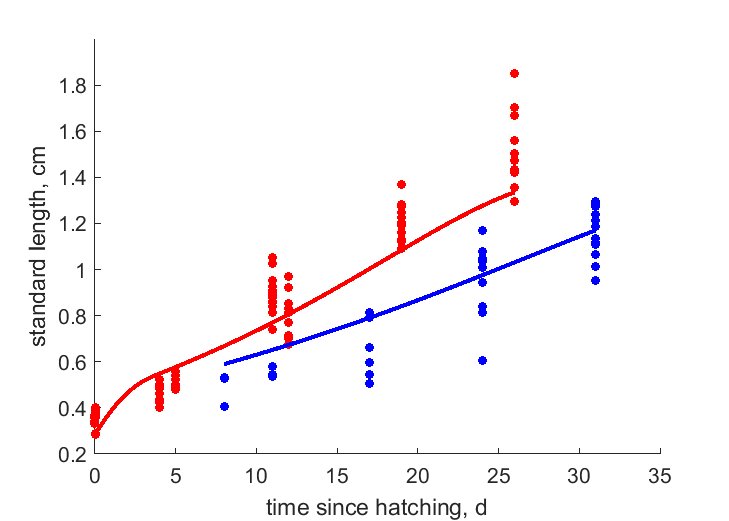
\includegraphics[width=1.0\textwidth]{figures/Chap4LarvaDataVSModel.png}
	\centering
	\caption{Simulated larval growth (lines) vs. larval growth of laboratory-reared \textit{E. ringens} individuals (dots) at a constant temperature of 14.5 \textdegree C (color blue) and 18.5 \textdegree C (color red) \citep{RiouOfel2021}. Age is expressed in days ($d$) after hatching and standard length in centimeters ($cm$).}
	\label{Chap4LarvaDataVSModel}
\end{figure}

\begin{figure}[H]
	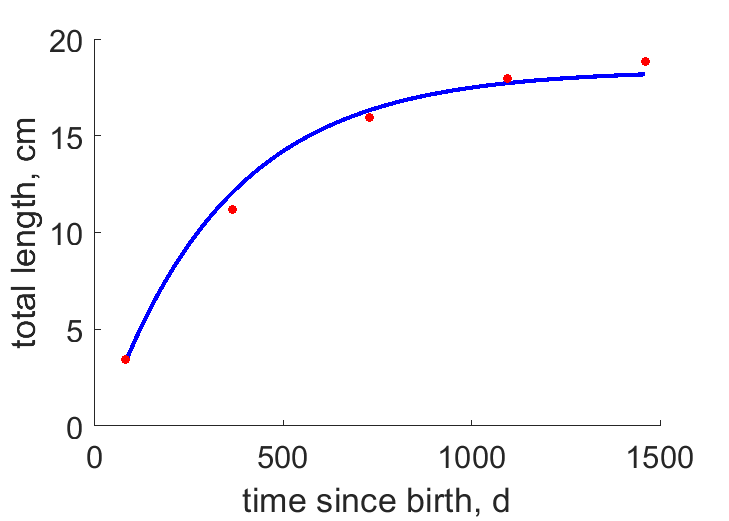
\includegraphics[width=1.0\textwidth]{figures/Chap4AdultDataVSModel.png}
	\centering
	\caption{Simulated DEB growth curve at 17 \textdegree C (blue line) vs. annual growth data (red dots) calculated from Von Bertalanffy parameters \citep{PaloMuck1987}. Age since birth is expressed in days ($d$) and total length in centimeters ($cm$).}
	\label{Chap4AdultDataVSModel}
\end{figure}

\begin{figure}[ht]
	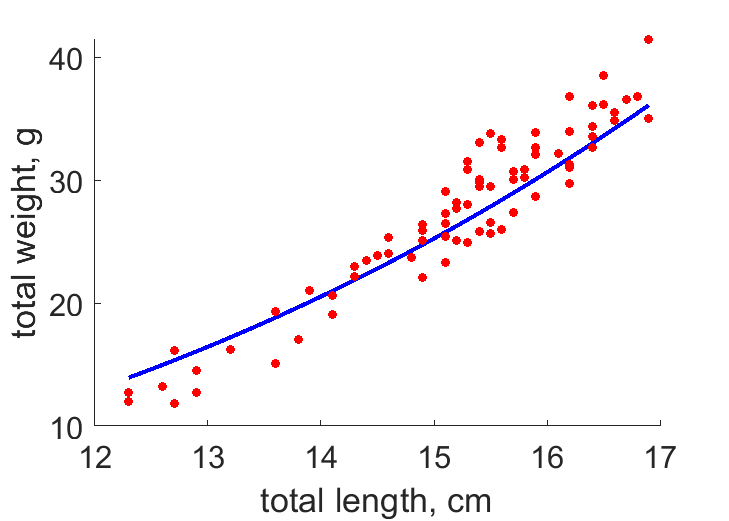
\includegraphics[width=1.0\textwidth]{figures/Chap4LengthVSWeight.png}
	\centering
	\caption{The relationship between total length ($cm$) and total weight ($g$) from the literature (red dots, \cite{Mina1968}) is compared to the values estimated by the DEB model (blue line).}
	\label{Chap4LengthVSWeight}
\end{figure}

\begin{figure}[H]
	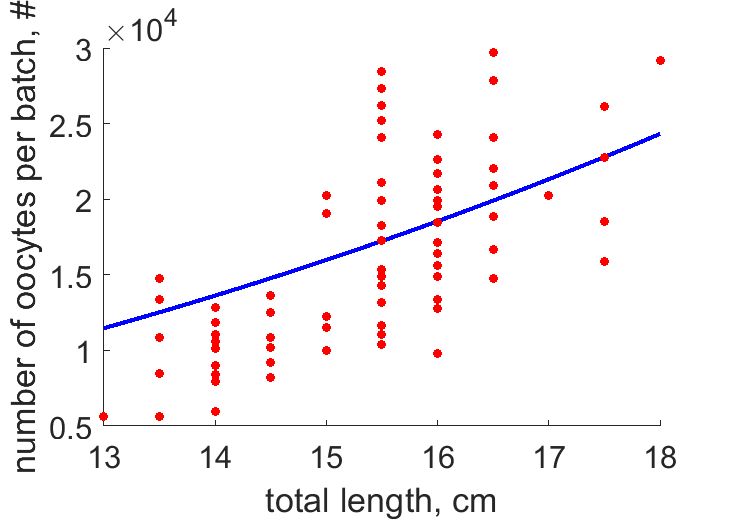
\includegraphics[width=1.0\textwidth]{figures/Chap4LengthVSOocytes.png}
	\centering
	\caption{Relationship between total length ($cm$) and number ($\#$) of oocytes per batch (red dots, \cite{PereBuit2000}) compared to the fitted values obtained by the DEB model (blue line).}
	\label{Chap4LengthVSOocytes}
\end{figure}

\subsection{Comparing the simulated growth of a standard and accelerated model}

In Chapter \ref{Chap3}, a standard \acrshort{deb} growth model was employed to simulate larval growth patterns in \textit{\gls{ringens}} developed by \cite{PethRoos2013}. This section will focus on a comparison of performance between the standard model ($DEB_{std}$) and a growth-accelerated model ($DEB_{abj}$) developed in this study. In all subsequent simulation experiments, the non-monotonic temperature correction curve (equation \ref{C_T}) as detailed in Table \ref{TabSimusChap3}, was employed.\\

Fig. \ref{Chap4DEBoutVSArturoLabf1V4} illustrates that the standard model exhibits a slight overestimation of larval growth, whereas the accelerated model accurately reflects the acceleration of growth rate during the early life stages, up to an age of 30 $days$ after hatching and a length of 2 $cm$ fitting well with larval growth data obtained from laboratory experiments at 15, 18 and 19 \textdegree C. A comparable performance was observed in both types of models up to five $days$ of age. Subsequently, the standard model demonstrated a nearly exponential increase in growth, whereas the accelerated model exhibited a higher fit to the data.\\

\begin{figure}[ht]
	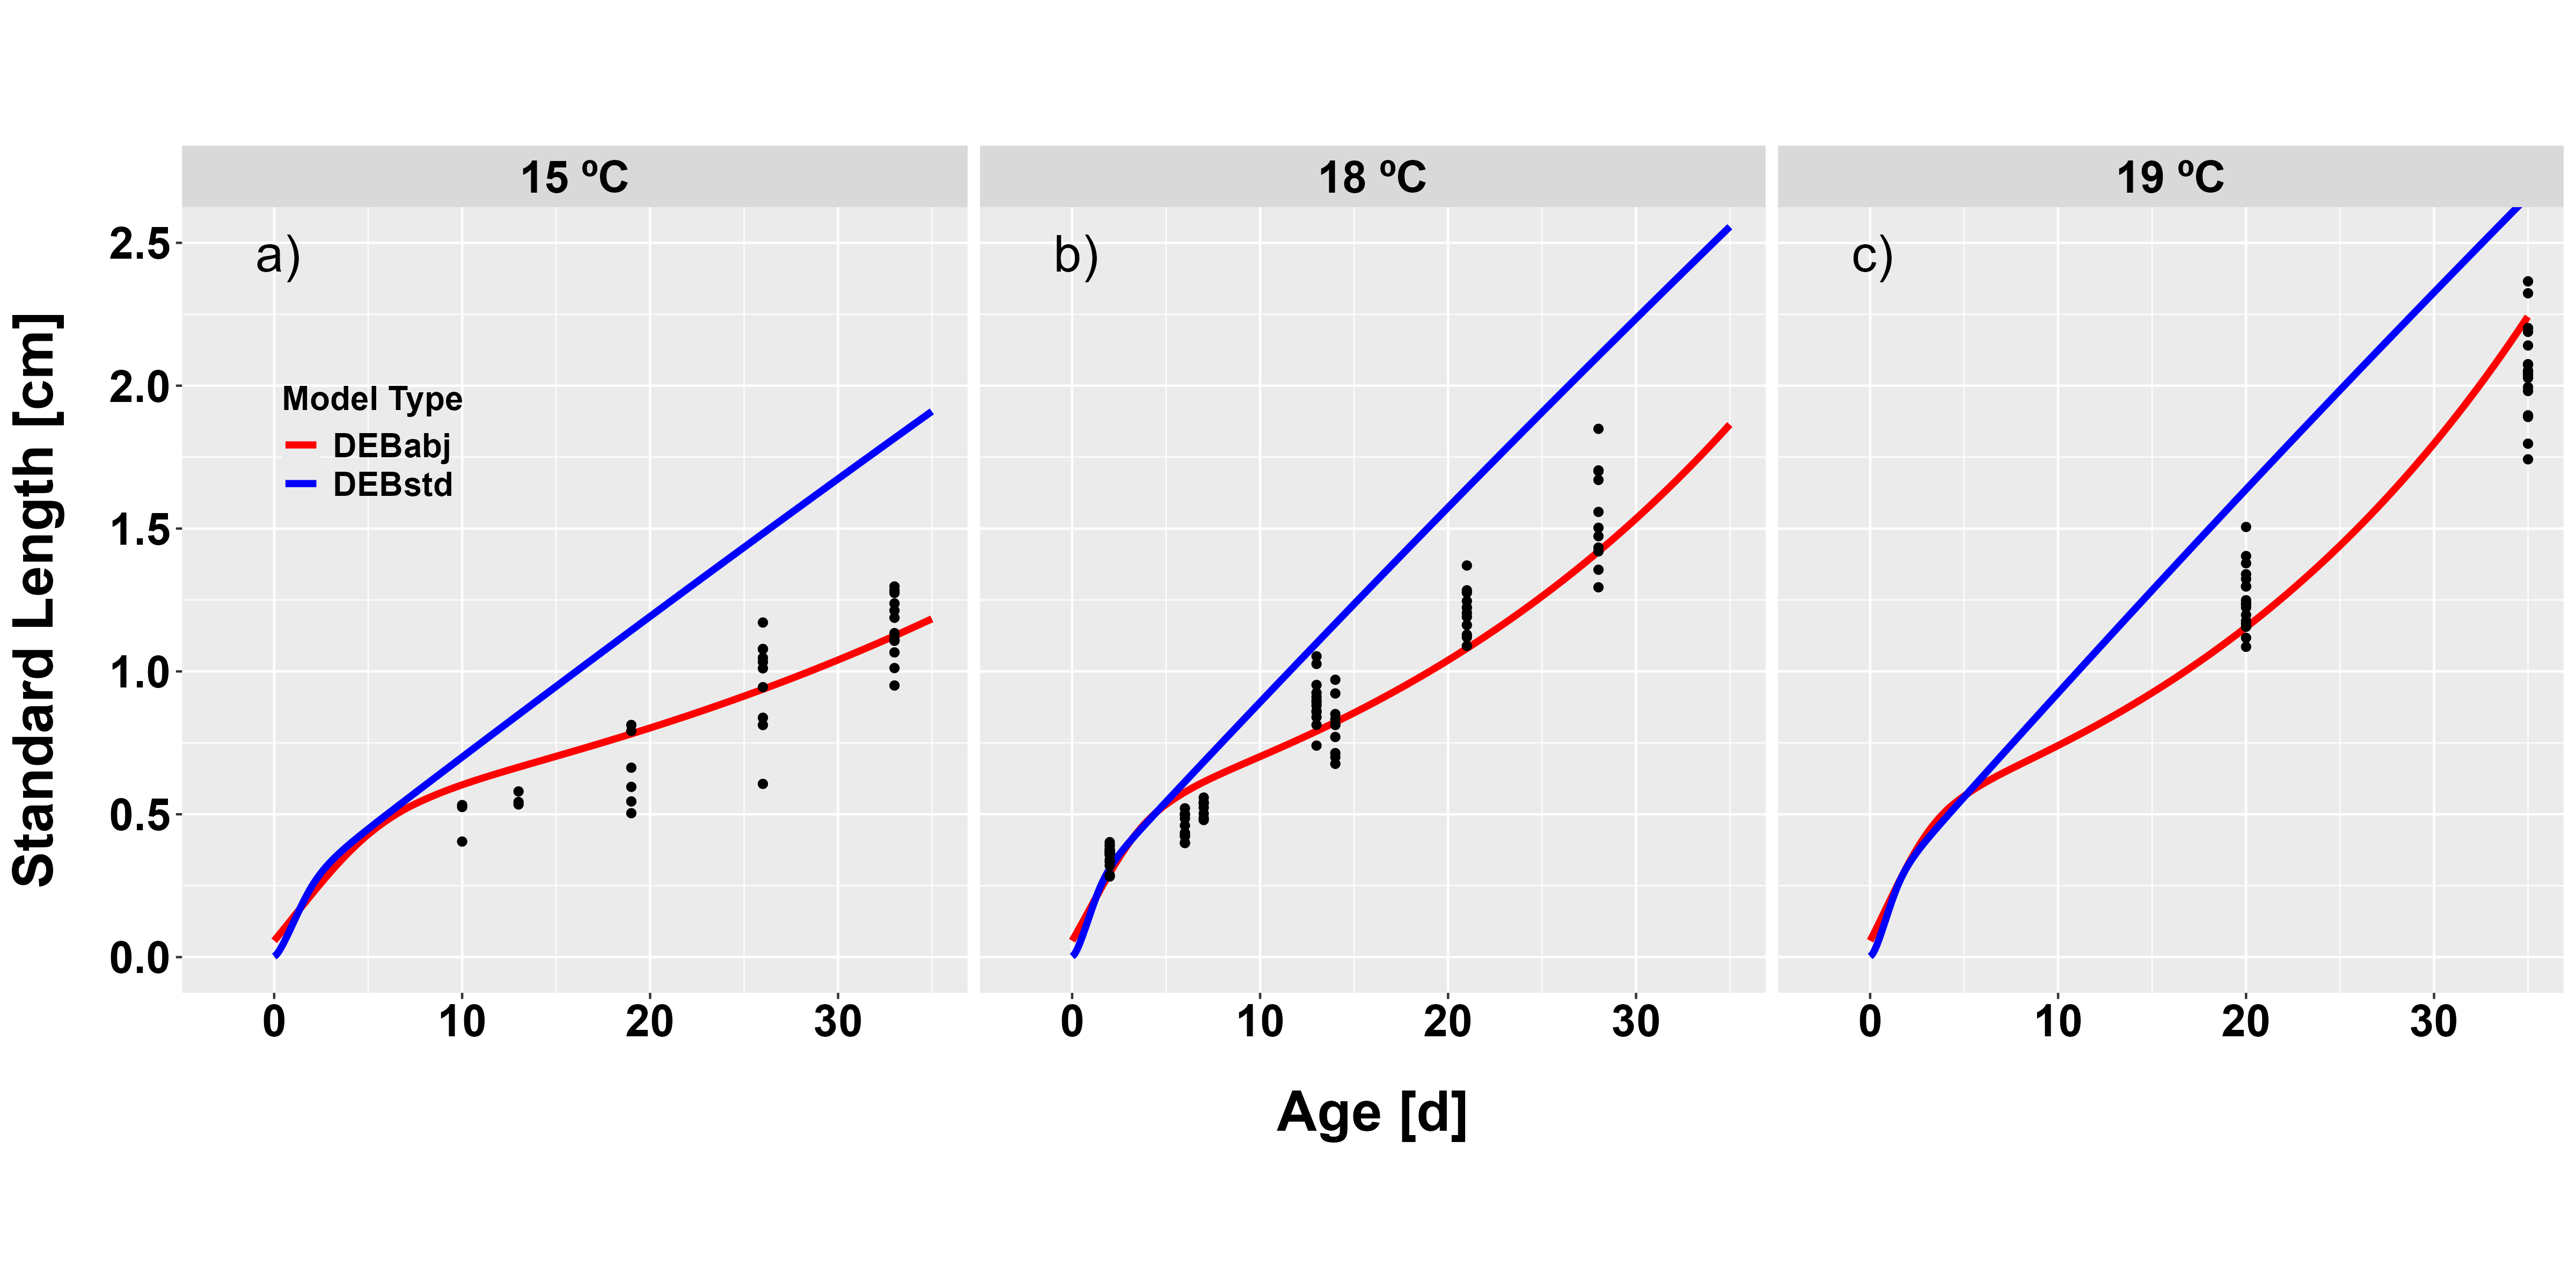
\includegraphics[width=1.0\textwidth]{figures/Chap4DEBoutVSArturoLabf1V4.png}
	\centering
	\caption{Comparison of simulated larval growth curves by $DEB_{std}$ model (blue line) and $DEB_{abj}$ model (red line) at different temperatures a) 15, c) 18 and c) 19 \textdegree C and laboratory growth observations (black dots) for \textit{E. ringens}. Temperature correction curve of Case 1 described in Table \ref{TabSimusChap3} was used.}
	\label{Chap4DEBoutVSArturoLabf1V4}
\end{figure}

In the $DEB_{abj}$ model, the transition sizes (birth, metamorphosis, and puberty) are based on estimated energy thresholds. The time (age) required to reach these thresholds varies with temperature. For the standard model ($DEB_{std}$), we have used the $DEB_{abj}$ sizes and calculated the age to reach each size. It should be noted that $DEB_{std}$ has no metamorphosis, for example. The experiments were limited to a range of temperature between 14 -21 \textdegree C (Fig. \ref{Chap4age_transitions2SPcTcase1}). This is because above this temperature, the time required to reach the transitions becomes disproportionately long. An increase in temperature could shorten the time at birth simulated by $DEB_{abj}$ even at temperatures above 19 \textdegree C compared to the predictions made by $DEB_{std}$.\\

\begin{figure}[ht]
	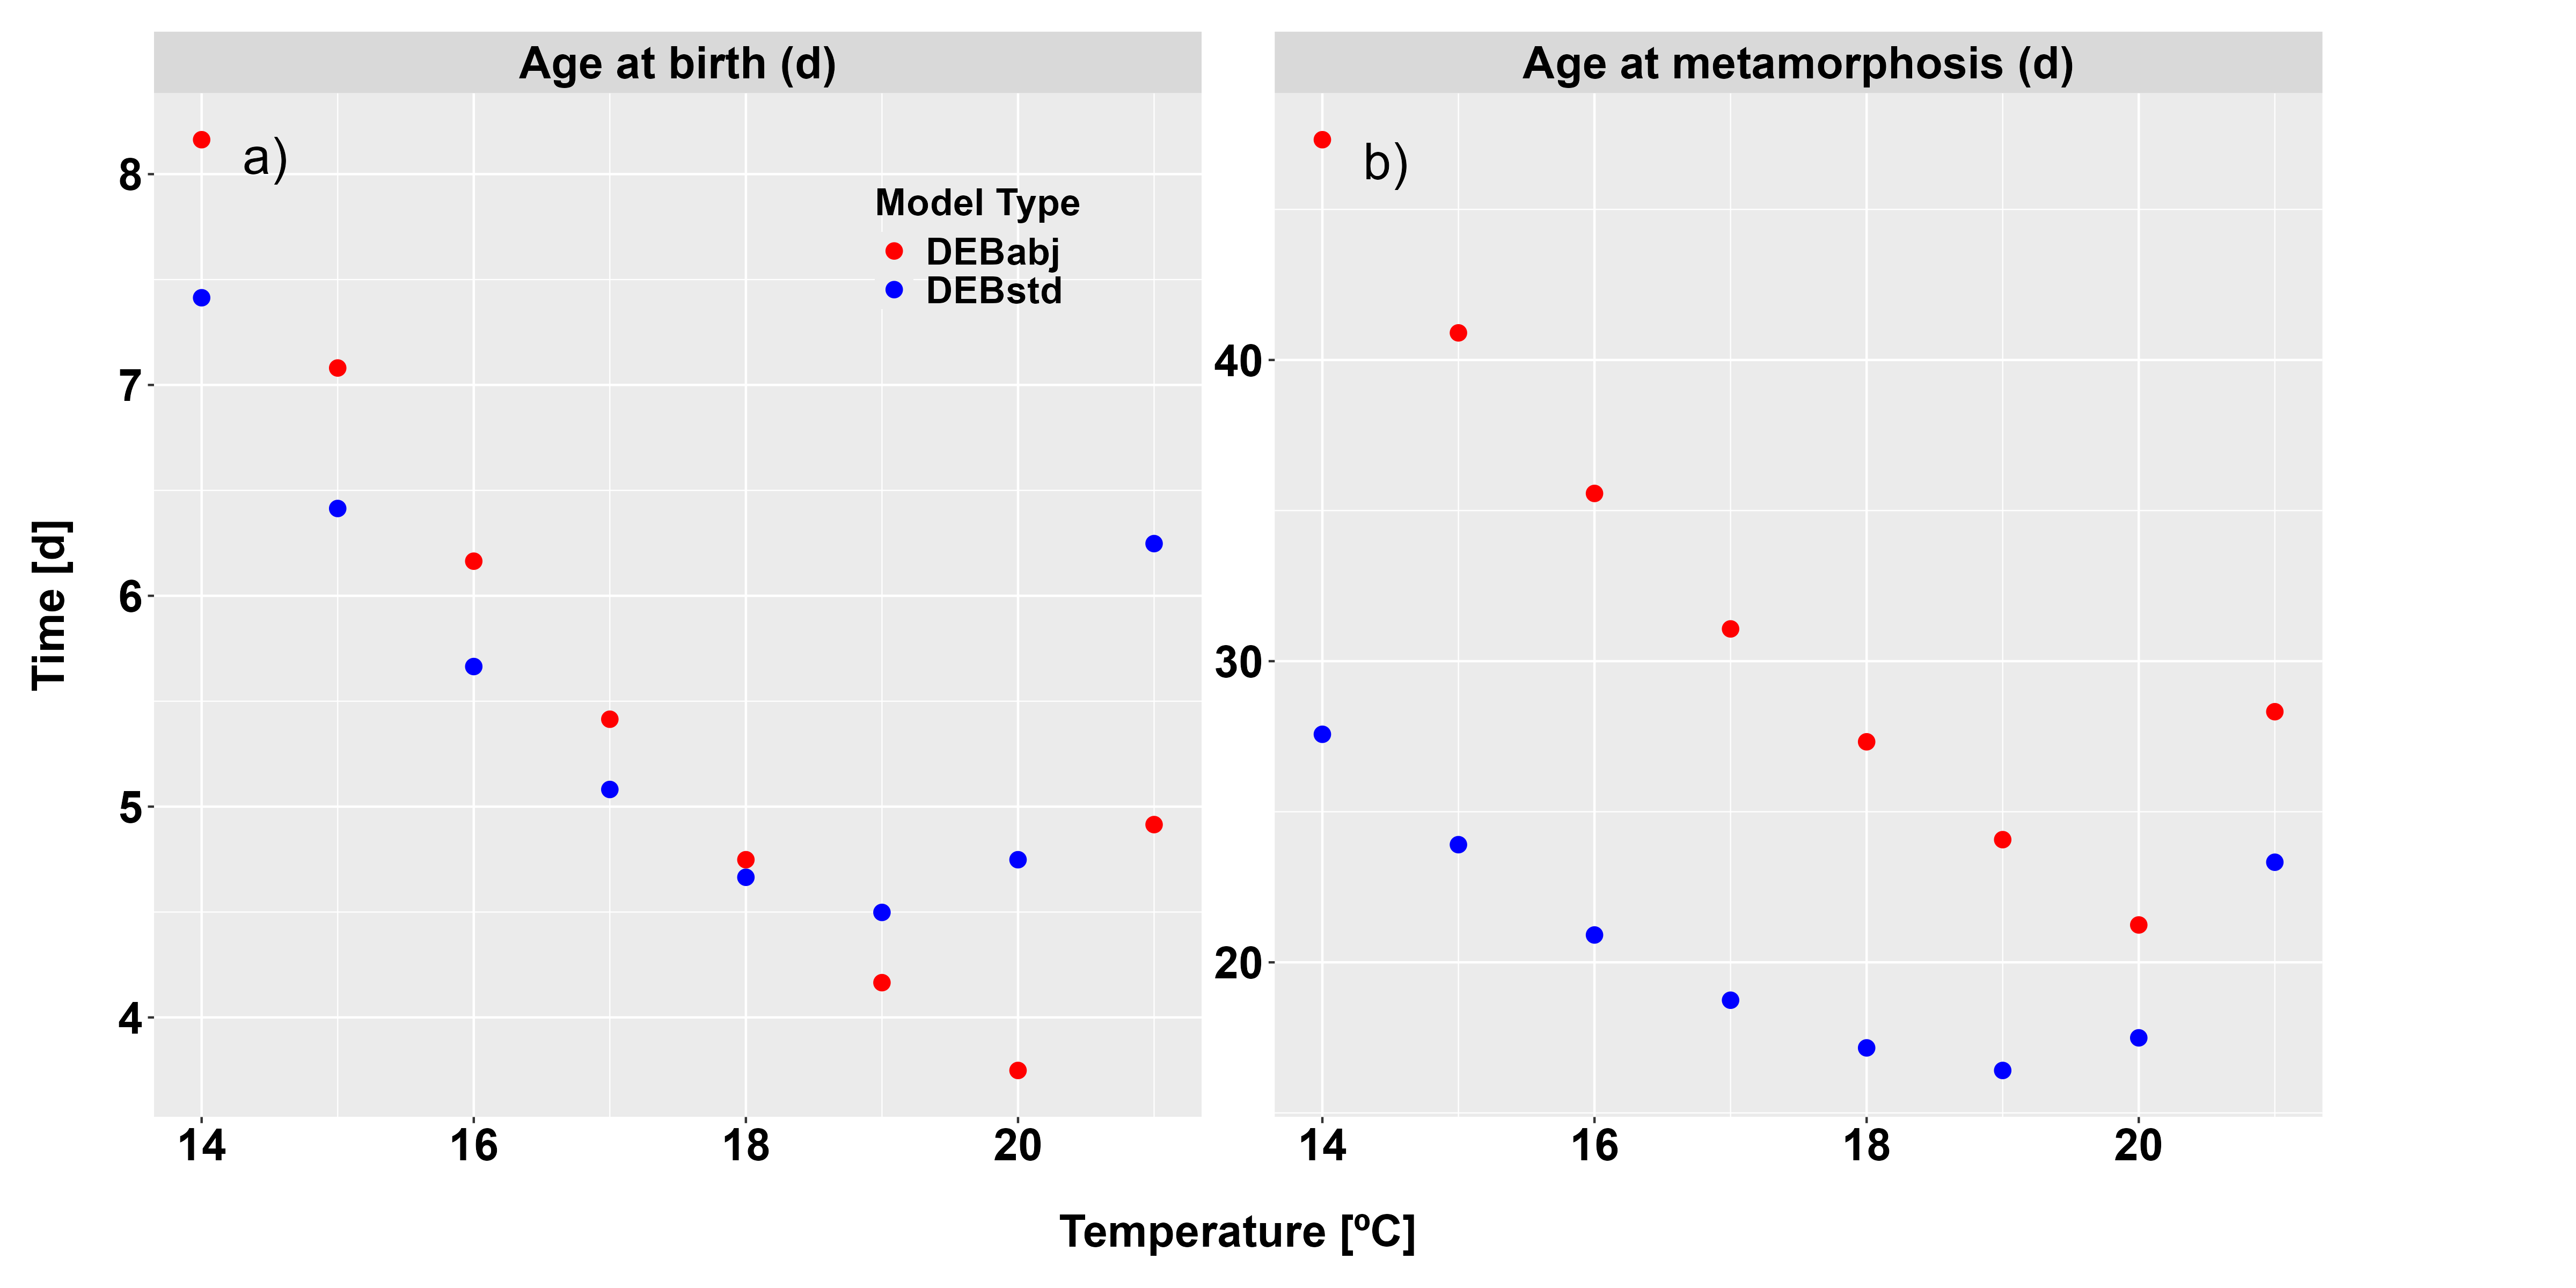
\includegraphics[width=1.0\textwidth]{figures/Chap4age_transitions2SPcTcase1.png}
	\centering
	\caption{Simulated a) Age at birth (first feeding) and b) age at metamorphosis (end of growth acceleration) by $DEB_{std}$ model (blue dots) and $DEB_{abj}$ model (red dots) in a temperature range between 14 and 21 \textdegree C using the temperature correction curve of Case 1 described in Table \ref{TabSimusChap3}}
	\label{Chap4age_transitions2SPcTcase1}
\end{figure}

For the starvation experiments on larvae of two different sizes (0.5 and 3 $cm$), in order to start with the same initial conditions, the reserve ($E$) of a each larval size at 20 \textdegree C was calculated. Subsequently, the functional response was set to a value of zero ($f = 0$) to simulate starvation. The number of days until this condition was reached was then calculated. In conducting these experiments (Fig. \ref{Chap4t_starvation_f0_V2cTcase1}), we utilized a temperature range of 14 to 30 \textdegree C, a range that encompasses the coastal regions off Peru, including those experiencing during El Ni\~{n}o events. Individuals inevitably reach a state of starvation due to the inability to pay maintenance costs. As a small larva (0.5 $cm$), $DEB_{abj}$ demonstrates greater resistance (in $days$) before reaching starvation. This characteristic is reversed for larger larvae (3 $cm$), where $DEB_{std}$ has the advantage.

\begin{figure}[ht]
	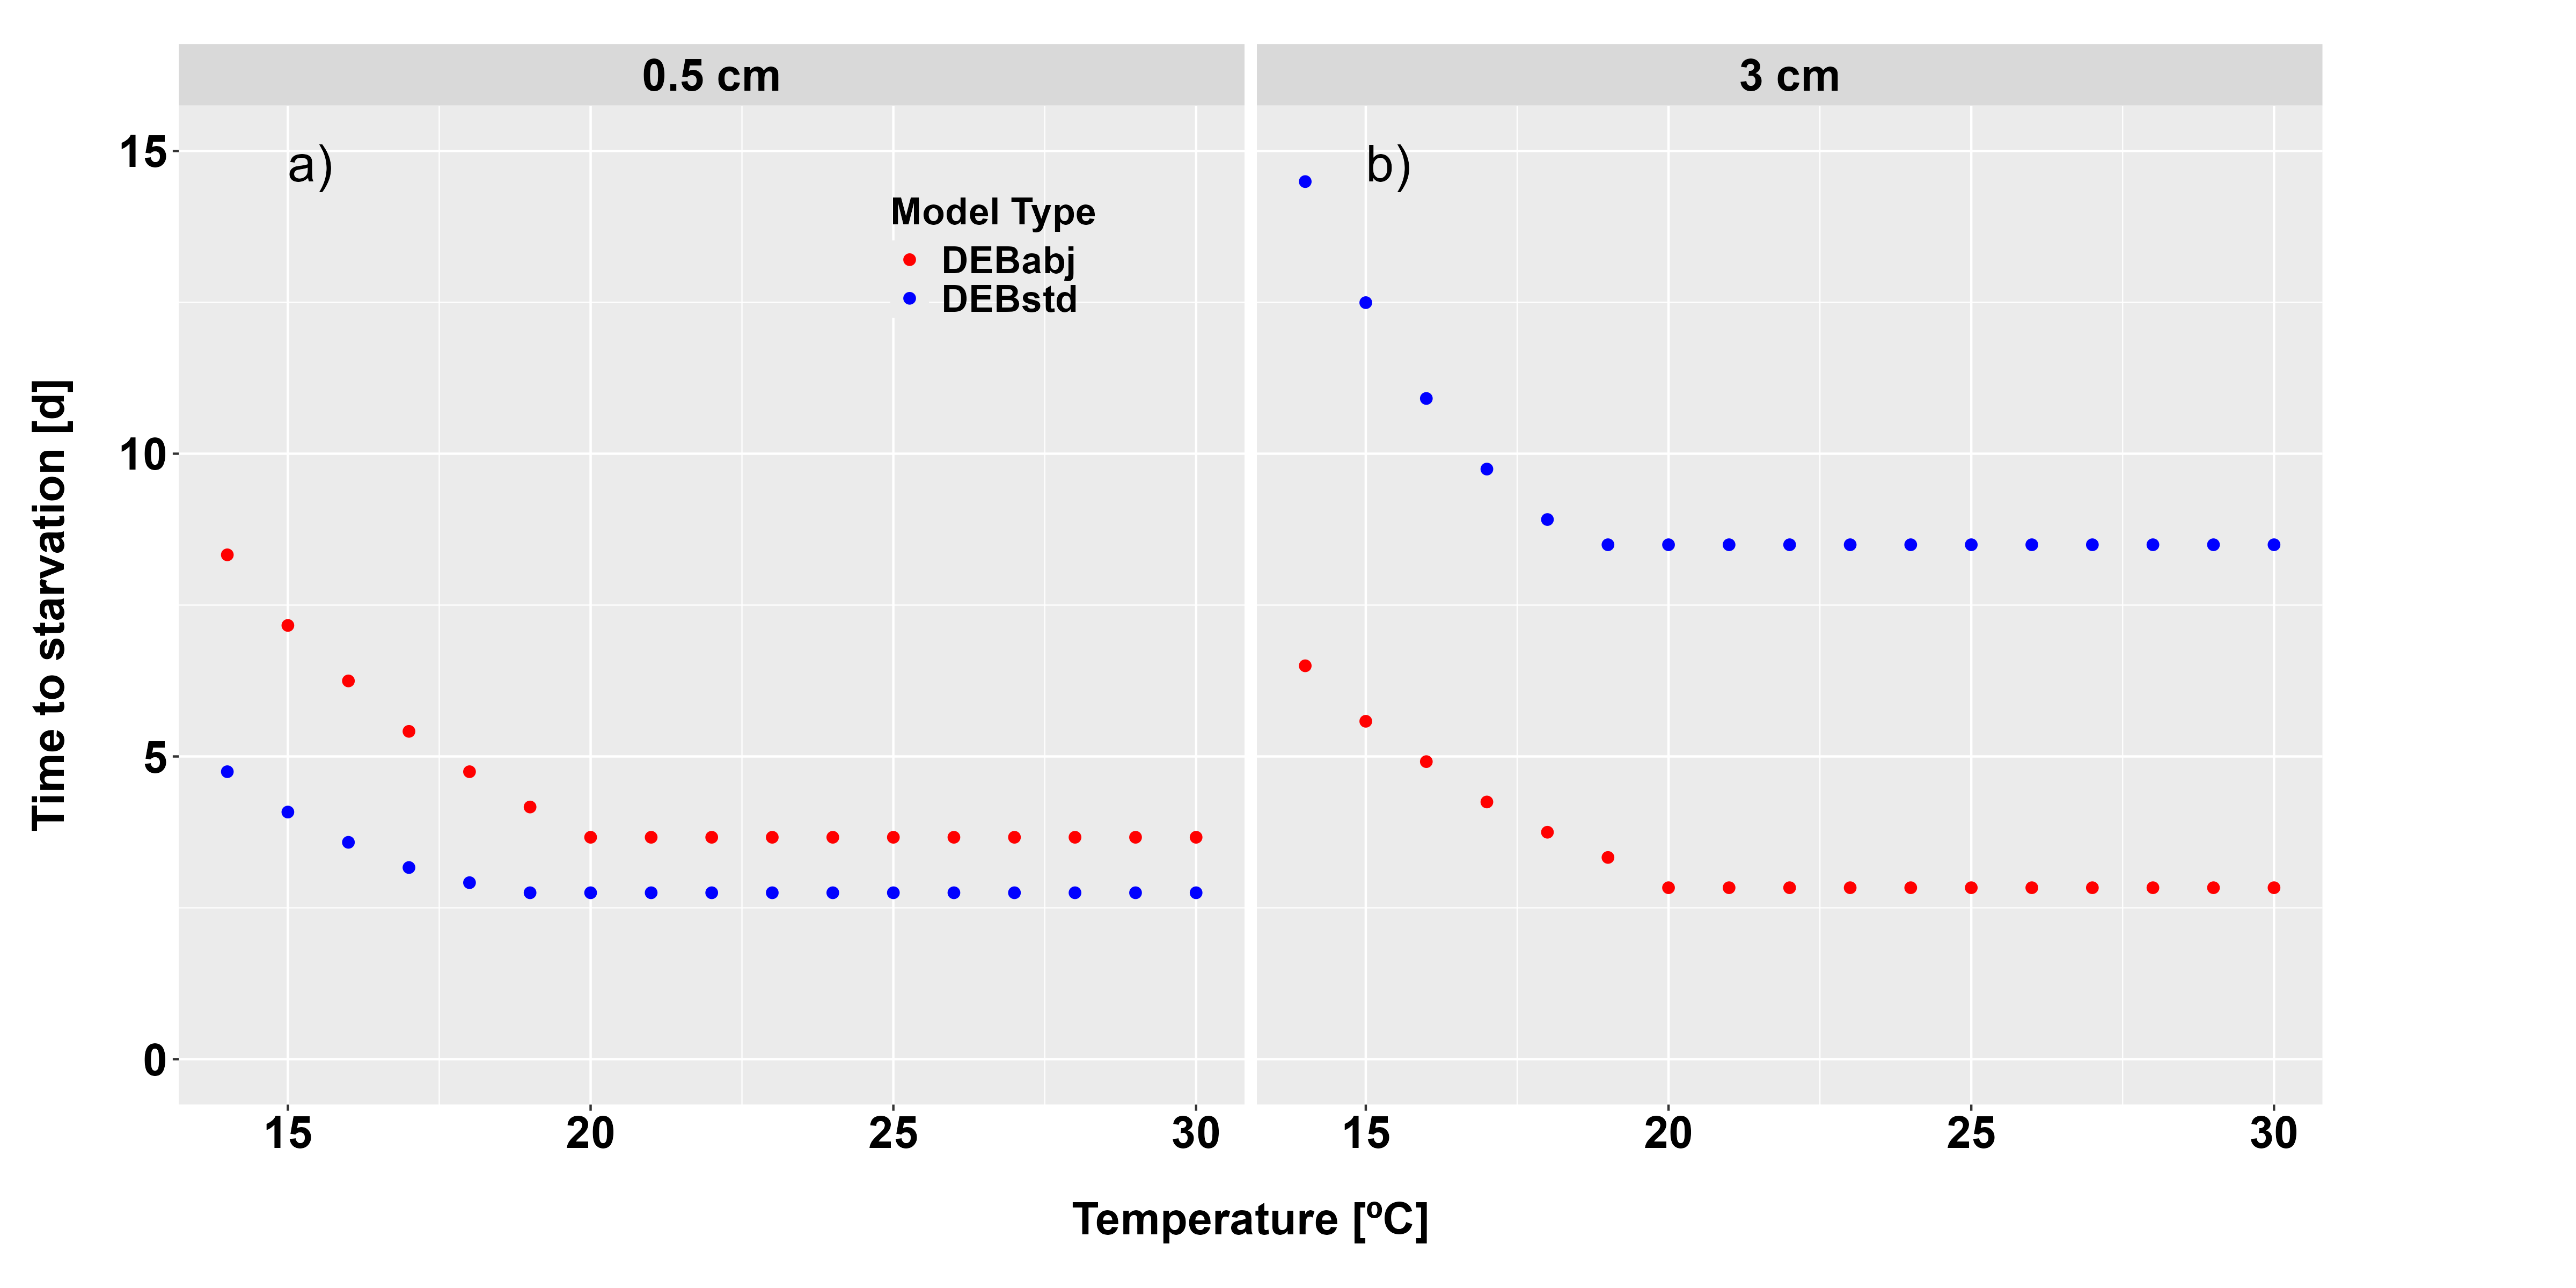
\includegraphics[width=1.0\textwidth]{figures/Chap4t_starvation_f0_V2cTcase1.png}
	\centering
	\caption{Simulated starvation experiments were conducted using $DEB_{std}$ model (blue dots) and $DEB_{abj}$ model (red dots) for two different larval sizes (a) $0.5 cm$ and b) $3 cm$) in a temperature range between 14 and 30 \textdegree C, with $f = 0$ (no feeding). Temperature correction curve of Case 1 described in Table \ref{TabSimusChap3} was used.}
	\label{Chap4t_starvation_f0_V2cTcase1}
\end{figure}

\section{Discussion}

List of bullet points are coming soon . . .